% Options for packages loaded elsewhere
\PassOptionsToPackage{unicode}{hyperref}
\PassOptionsToPackage{hyphens}{url}
\PassOptionsToPackage{dvipsnames,svgnames,x11names}{xcolor}
%
\documentclass[
]{article}

\usepackage{amsmath,amssymb}
\usepackage{iftex}
\ifPDFTeX
  \usepackage[T1]{fontenc}
  \usepackage[utf8]{inputenc}
  \usepackage{textcomp} % provide euro and other symbols
\else % if luatex or xetex
  \usepackage{unicode-math}
  \defaultfontfeatures{Scale=MatchLowercase}
  \defaultfontfeatures[\rmfamily]{Ligatures=TeX,Scale=1}
\fi
\usepackage{lmodern}
\ifPDFTeX\else  
    % xetex/luatex font selection
\fi
% Use upquote if available, for straight quotes in verbatim environments
\IfFileExists{upquote.sty}{\usepackage{upquote}}{}
\IfFileExists{microtype.sty}{% use microtype if available
  \usepackage[]{microtype}
  \UseMicrotypeSet[protrusion]{basicmath} % disable protrusion for tt fonts
}{}
\makeatletter
\@ifundefined{KOMAClassName}{% if non-KOMA class
  \IfFileExists{parskip.sty}{%
    \usepackage{parskip}
  }{% else
    \setlength{\parindent}{0pt}
    \setlength{\parskip}{6pt plus 2pt minus 1pt}}
}{% if KOMA class
  \KOMAoptions{parskip=half}}
\makeatother
\usepackage{xcolor}
\setlength{\emergencystretch}{3em} % prevent overfull lines
\setcounter{secnumdepth}{5}
% Make \paragraph and \subparagraph free-standing
\ifx\paragraph\undefined\else
  \let\oldparagraph\paragraph
  \renewcommand{\paragraph}[1]{\oldparagraph{#1}\mbox{}}
\fi
\ifx\subparagraph\undefined\else
  \let\oldsubparagraph\subparagraph
  \renewcommand{\subparagraph}[1]{\oldsubparagraph{#1}\mbox{}}
\fi


\providecommand{\tightlist}{%
  \setlength{\itemsep}{0pt}\setlength{\parskip}{0pt}}\usepackage{longtable,booktabs,array}
\usepackage{calc} % for calculating minipage widths
% Correct order of tables after \paragraph or \subparagraph
\usepackage{etoolbox}
\makeatletter
\patchcmd\longtable{\par}{\if@noskipsec\mbox{}\fi\par}{}{}
\makeatother
% Allow footnotes in longtable head/foot
\IfFileExists{footnotehyper.sty}{\usepackage{footnotehyper}}{\usepackage{footnote}}
\makesavenoteenv{longtable}
\usepackage{graphicx}
\makeatletter
\def\maxwidth{\ifdim\Gin@nat@width>\linewidth\linewidth\else\Gin@nat@width\fi}
\def\maxheight{\ifdim\Gin@nat@height>\textheight\textheight\else\Gin@nat@height\fi}
\makeatother
% Scale images if necessary, so that they will not overflow the page
% margins by default, and it is still possible to overwrite the defaults
% using explicit options in \includegraphics[width, height, ...]{}
\setkeys{Gin}{width=\maxwidth,height=\maxheight,keepaspectratio}
% Set default figure placement to htbp
\makeatletter
\def\fps@figure{htbp}
\makeatother
\newlength{\cslhangindent}
\setlength{\cslhangindent}{1.5em}
\newlength{\csllabelwidth}
\setlength{\csllabelwidth}{3em}
\newlength{\cslentryspacingunit} % times entry-spacing
\setlength{\cslentryspacingunit}{\parskip}
\newenvironment{CSLReferences}[2] % #1 hanging-ident, #2 entry spacing
 {% don't indent paragraphs
  \setlength{\parindent}{0pt}
  % turn on hanging indent if param 1 is 1
  \ifodd #1
  \let\oldpar\par
  \def\par{\hangindent=\cslhangindent\oldpar}
  \fi
  % set entry spacing
  \setlength{\parskip}{#2\cslentryspacingunit}
 }%
 {}
\usepackage{calc}
\newcommand{\CSLBlock}[1]{#1\hfill\break}
\newcommand{\CSLLeftMargin}[1]{\parbox[t]{\csllabelwidth}{#1}}
\newcommand{\CSLRightInline}[1]{\parbox[t]{\linewidth - \csllabelwidth}{#1}\break}
\newcommand{\CSLIndent}[1]{\hspace{\cslhangindent}#1}

\usepackage{fontspec}
\usepackage{xcolor}
\setmainfont{Arial}
\usepackage{anyfontsize}
\fontsize{12}{18}\selectfont
\usepackage{booktabs}
\usepackage{graphicx}
\usepackage[nottoc]{tocbibind}
\usepackage{natbib}
\renewcommand{\bibsection}{}
\usepackage[a4paper, top=2.5cm, bottom=3cm, left=2.5cm, right=2.5cm]{geometry}
\usepackage{tocloft}
\renewcommand{\cftsecleader}{\cftdotfill{\cftdotsep}}
\makeatletter
\makeatother
\makeatletter
\makeatother
\makeatletter
\@ifpackageloaded{caption}{}{\usepackage{caption}}
\AtBeginDocument{%
\ifdefined\contentsname
  \renewcommand*\contentsname{Table of contents}
\else
  \newcommand\contentsname{Table of contents}
\fi
\ifdefined\listfigurename
  \renewcommand*\listfigurename{List of Figures}
\else
  \newcommand\listfigurename{List of Figures}
\fi
\ifdefined\listtablename
  \renewcommand*\listtablename{List of Tables}
\else
  \newcommand\listtablename{List of Tables}
\fi
\ifdefined\figurename
  \renewcommand*\figurename{Figure}
\else
  \newcommand\figurename{Figure}
\fi
\ifdefined\tablename
  \renewcommand*\tablename{Table}
\else
  \newcommand\tablename{Table}
\fi
}
\@ifpackageloaded{float}{}{\usepackage{float}}
\floatstyle{ruled}
\@ifundefined{c@chapter}{\newfloat{codelisting}{h}{lop}}{\newfloat{codelisting}{h}{lop}[chapter]}
\floatname{codelisting}{Listing}
\newcommand*\listoflistings{\listof{codelisting}{List of Listings}}
\makeatother
\makeatletter
\@ifpackageloaded{caption}{}{\usepackage{caption}}
\@ifpackageloaded{subcaption}{}{\usepackage{subcaption}}
\makeatother
\makeatletter
\@ifpackageloaded{tcolorbox}{}{\usepackage[skins,breakable]{tcolorbox}}
\makeatother
\makeatletter
\@ifundefined{shadecolor}{\definecolor{shadecolor}{rgb}{.97, .97, .97}}
\makeatother
\makeatletter
\makeatother
\makeatletter
\makeatother
\ifLuaTeX
  \usepackage{selnolig}  % disable illegal ligatures
\fi
\IfFileExists{bookmark.sty}{\usepackage{bookmark}}{\usepackage{hyperref}}
\IfFileExists{xurl.sty}{\usepackage{xurl}}{} % add URL line breaks if available
\urlstyle{same} % disable monospaced font for URLs
\hypersetup{
  colorlinks=true,
  linkcolor={black},
  filecolor={Maroon},
  citecolor={Blue},
  urlcolor={Blue},
  pdfcreator={LaTeX via pandoc}}

\author{}
\date{}

\begin{document}
\ifdefined\Shaded\renewenvironment{Shaded}{\begin{tcolorbox}[boxrule=0pt, breakable, borderline west={3pt}{0pt}{shadecolor}, sharp corners, interior hidden, enhanced, frame hidden]}{\end{tcolorbox}}\fi

\begin{titlepage}
    \centering
    {\fontsize{12}{10}\selectfont ZURICH UNIVERSITY OF APPLIED SCIENCES\par}
    {\fontsize{12}{10}\selectfont SCHOOL OF LIFE SCIENCES AND FACILITY MANAGEMENT\par}
    {\fontsize{12}{10}\selectfont INSTITUTE OF NATURAL RESOURCE SCIENCES\par}
    \vspace{6cm}
    {\fontsize{14}{16}\bfseries Quantification of deforestation on Borneo in the last 20 years based on open source geodata\par}
    {\fontsize{12}{14}\bfseries Bachelor Thesis\par}
    {\fontsize{12}{14}\selectfont HS23\par}
    \vspace{2cm}
    {\fontsize{12}{14}\bfseries by\par}
    {\fontsize{12}{14}\bfseries Robin Pfaff\par}
    {\fontsize{12}{14}\selectfont BSc Environmental engineering\par}
    \vspace{2cm}
    {\fontsize{12}{14}\selectfont Submission date: \textcolor{red}{dd.mm}.2023\par}

    \vfill
    \begin{flushleft}
        1\textsuperscript{st} supervisor:\\
        Ochsner, Pascal\\
        2\textsuperscript{nd} supervisor:\\
        Ratnaweera, Nils\\
        ZHAW IUNR Research Group for Geoinformatics
    \end{flushleft}
\end{titlepage}

\newpage

\thispagestyle{empty}
\vspace*{\fill}

\hypertarget{imprint}{%
\section*{Imprint}\label{imprint}}

\vspace{0.5cm}

\textbf{Institute}\\
Institute of Natural Resource Sciences

\textbf{Form of citation}\\
APA 7th edition

\textbf{Keywords}\\
Alooideae, genetic diversity, in-silico, sequence alignment

\newpage

\hypertarget{abstract}{%
\section*{Abstract}\label{abstract}}

\thispagestyle{empty}

Lorem ipsum dolor sit amet, consectetur adipiscing elit. Curabitur nec
ipsum sit amet arcu blandit vulputate at sed felis. Nam auctor tortor in
risus aliquet, id interdum elit vestibulum. Nulla aliquam faucibus
purus, non laoreet mi sollicitudin id. Aliquam volutpat, ex eu pharetra
gravida, lacus nisl dictum ipsum, ac aliquam metus urna id leo. In
tristique risus ac finibus fringilla. Nullam vulputate enim id consequat
faucibus. Duis pellentesque metus ac fermentum auctor. Nam semper
tincidunt purus, nec volutpat mauris feugiat ut. Phasellus consectetur,
leo vitae facilisis dignissim, purus justo volutpat felis, vel efficitur
est orci sed mi.

Phasellus a nisi lacus. Nullam congue ultrices ex, sed lacinia massa
mattis sit amet. Nam fermentum, turpis ut congue viverra, nisl nunc
ultricies mauris, nec consequat turpis metus eget ligula. Aliquam erat
volutpat. Vivamus tempus nisl in est ultrices varius. Nunc nec purus
dolor. Sed a ullamcorper ex. Pellentesque habitant morbi tristique
senectus et netus et malesuada fames ac turpis egestas.

Lorem ipsum dolor sit amet, consectetur adipiscing elit. Curabitur nec
ipsum sit amet arcu blandit vulputate at sed felis. Nam auctor tortor in
risus aliquet, id interdum elit vestibulum. Nulla aliquam faucibus
purus, non laoreet mi sollicitudin id. Aliquam volutpat, ex eu pharetra
gravida, lacus nisl dictum ipsum, ac aliquam metus urna id leo. In
tristique risus ac finibus fringilla. Nullam vulputate enim id consequat
faucibus. Duis pellentesque metus ac fermentum auctor. Nam semper
tincidunt purus, nec volutpat mauris feugiat ut. Phasellus consectetur,
leo vitae facilisis dignissim, purus justo volutpat felis, vel efficitur
est orci sed mi.

Phasellus a nisi lacus. Nullam congue ultrices ex, sed lacinia massa
mattis sit amet. Nam fermentum, turpis ut congue viverra, nisl nunc
ultricies mauris, nec consequat turpis metus eget ligula. Aliquam erat
volutpat. Vivamus tempus nisl in est ultrices varius. Nunc nec purus
dolor. Sed a ullamcorper ex. Pellentesque habitant morbi tristique
senectus et netus et malesuada fames ac turpis egestas.

\newpage
\tableofcontents
\newpage

\hypertarget{introduction}{%
\section{Introduction}\label{introduction}}

Lorem ipsum dolor sit amet, consectetur adipiscing elit. Donec at ante
ut lectus tempor viverra vitae vel leo. Fusce maximus libero eu semper
pharetra. Quisque tristique, mauris vel consectetur lobortis, metus
ligula gravida metus, id commodo turpis turpis nec
dolor(Table~\ref{tbl-mytable1}).

\begin{figure}

{\centering 
\includegraphics[width=0.5\textwidth,height=\textheight]{placeholder.jpg}

}

\caption{Example Picture 1}

\end{figure}

For more information, refer to the literature review(Chapman et al.,
\protect\hyperlink{ref-chapmanCompoundingImpactDeforestation2020}{2020};
Descals et al.,
\protect\hyperlink{ref-descalsHighresolutionGlobalMap2021}{2021}).

\hypertarget{tbl-mytable1}{}
\begin{longtable}[]{@{}lrr@{}}
\caption{\label{tbl-mytable1}My caption}\tabularnewline
\toprule\noalign{}
Car & MPG & Cylinders \\
\midrule\noalign{}
\endfirsthead
\toprule\noalign{}
Car & MPG & Cylinders \\
\midrule\noalign{}
\endhead
\bottomrule\noalign{}
\endlastfoot
Mazda RX4 & 21 & 6 \\
Mazda RX4 Wag & 21 & 6 \\
Datsun 710 & 22.8 & 4 \\
Hornet 4 Drive & 21.4 & 6 \\
\end{longtable}

Lorem ipsum dolor sit amet, consectetur adipiscing elit. Donec at ante
ut lectus tempor viverra vitae vel leo. Fusce maximus libero eu semper
pharetra. Quisque tristique, mauris vel consectetur lobortis, metus
ligula gravida metus, id commodo turpis turpis nec dolor.

\begin{figure}


\includegraphics[width=0.5\textwidth,height=\textheight]{placeholder.jpg} \hfill{}

\caption{Example Picture on the left}

\end{figure}

Lorem ipsum dolor sit amet, consectetur adipiscing elit. Curabitur nec
ipsum sit amet arcu blandit vulputate at sed felis. Nam auctor tortor in
risus aliquet, id interdum elit vestibulum. Nulla aliquam faucibus
purus, non laoreet mi sollicitudin id. Aliquam volutpat, ex eu pharetra
gravida, lacus nisl dictum ipsum, ac aliquam metus urna id leo. In
tristique risus ac finibus fringilla. Nullam vulputate enim id consequat
faucibus. Duis pellentesque metus ac fermentum auctor. Nam semper
tincidunt purus, nec volutpat mauris feugiat ut. Phasellus consectetur,
leo vitae facilisis dignissim, purus justo volutpat felis, vel efficitur
est orci sed mi.

Phasellus a nisi lacus. Nullam congue ultrices ex, sed lacinia massa
mattis sit amet. Nam fermentum, turpis ut congue viverra, nisl nunc
ultricies mauris, nec consequat turpis metus eget ligula. Aliquam erat
volutpat. Vivamus tempus nisl in est ultrices varius. Nunc nec purus
dolor. Sed a ullamcorper ex. Pellentesque habitant morbi tristique
senectus et netus et malesuada fames ac turpis egestas.

Lorem ipsum dolor sit amet, consectetur adipiscing elit. Curabitur nec
ipsum sit amet arcu blandit vulputate at sed felis. Nam auctor tortor in
risus aliquet, id interdum elit vestibulum. Nulla aliquam faucibus
purus, non laoreet mi sollicitudin id. Aliquam volutpat, ex eu pharetra
gravida, lacus nisl dictum ipsum, ac aliquam metus urna id leo. In
tristique risus ac finibus fringilla. Nullam vulputate enim id consequat
faucibus. Duis pellentesque metus ac fermentum auctor. Nam semper
tincidunt purus, nec volutpat mauris feugiat ut. Phasellus consectetur,
leo vitae facilisis dignissim, purus justo volutpat felis, vel efficitur
est orci sed mi.

Phasellus a nisi lacus. Nullam congue ultrices ex, sed lacinia massa
mattis sit amet. Nam fermentum, turpis ut congue viverra, nisl nunc
ultricies mauris, nec consequat turpis metus eget ligula. Aliquam erat
volutpat. Vivamus tempus nisl in est ultrices varius. Nunc nec purus
dolor. Sed a ullamcorper ex. Pellentesque habitant morbi tristique
senectus et netus et malesuada fames ac turpis egestas.

Figure @ref(fig-my-diagram)

\begin{figure}[H]

{\centering 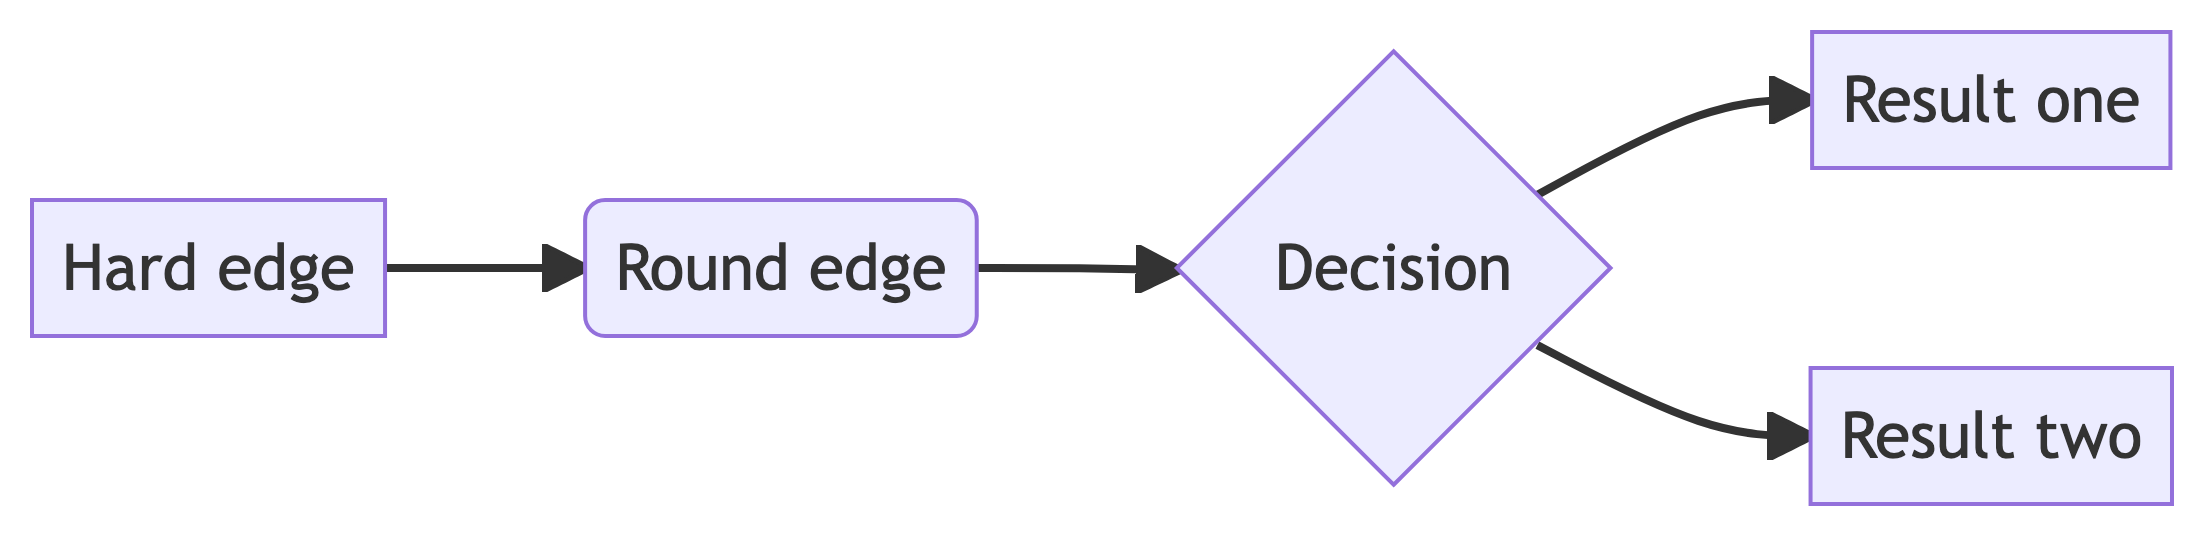
\includegraphics[width=5.74in,height=1.4in]{Main_files/figure-latex/mermaid-figure-1.png}

}

\end{figure}

\hypertarget{literature-review}{%
\section{Literature review}\label{literature-review}}

\hypertarget{rspo}{%
\subsection{RSPO}\label{rspo}}

Lorem ipsum dolor sit amet, consectetur adipiscing elit. Donec at ante
ut lectus tempor viverra vitae vel leo. Fusce maximus libero eu semper
pharetra. Quisque tristique, mauris vel consectetur lobortis, metus
ligula gravida metus, id commodo turpis turpis nec dolor
(Table~\ref{tbl-mytable2}).

\begin{figure}

{\centering 
\includegraphics[width=0.5\textwidth,height=\textheight]{placeholder.jpg}

}

\caption{Example Picture 2}

\end{figure}

For more information, refer to the literature review (Chapman et al.,
\protect\hyperlink{ref-chapmanCompoundingImpactDeforestation2020}{2020};
Descals et al.,
\protect\hyperlink{ref-descalsHighresolutionGlobalMap2021}{2021}).

\hypertarget{tbl-mytable2}{}
\begin{longtable}[]{@{}lrr@{}}
\caption{\label{tbl-mytable2}mycaption}\tabularnewline
\toprule\noalign{}
Car & MPG & Cylinders \\
\midrule\noalign{}
\endfirsthead
\toprule\noalign{}
Car & MPG & Cylinders \\
\midrule\noalign{}
\endhead
\bottomrule\noalign{}
\endlastfoot
Mazda RX4 & 21 & 6 \\
Mazda RX4 Wag & 21 & 6 \\
Datsun 710 & 22.8 & 4 \\
Hornet 4 Drive & 21.4 & 6 \\
\end{longtable}

Lorem ipsum dolor sit amet, consectetur adipiscing elit. Donec at ante
ut lectus tempor viverra vitae vel leo. Fusce maximus libero eu semper
pharetra. Quisque tristique, mauris vel consectetur lobortis, metus
ligula gravida metus, id commodo turpis turpis nec dolor.

\begin{figure}


\includegraphics[width=0.5\textwidth,height=\textheight]{placeholder.jpg} \hfill{}

\caption{Example Picture on the left}

\end{figure}

\hypertarget{deforestation}{%
\subsection{Deforestation}\label{deforestation}}

Lorem ipsum dolor sit amet, consectetur adipiscing elit. Curabitur nec
ipsum sit amet arcu blandit vulputate at sed felis. Nam auctor tortor in
risus aliquet, id interdum elit vestibulum. Nulla aliquam faucibus
purus, non laoreet mi sollicitudin id. Aliquam volutpat, ex eu pharetra
gravida, lacus nisl dictum ipsum, ac aliquam metus urna id leo. In
tristique risus ac finibus fringilla. Nullam vulputate enim id consequat
faucibus. Duis pellentesque metus ac fermentum auctor. Nam semper
tincidunt purus, nec volutpat mauris feugiat ut. Phasellus consectetur,
leo vitae facilisis dignissim, purus justo volutpat felis, vel efficitur
est orci sed mi.

\hypertarget{infrastructure}{%
\subsection{Infrastructure}\label{infrastructure}}

Phasellus a nisi lacus. Nullam congue ultrices ex, sed lacinia massa
mattis sit amet. Nam fermentum, turpis ut congue viverra, nisl nunc
ultricies mauris, nec consequat turpis metus eget ligula. Aliquam erat
volutpat. Vivamus tempus nisl in est ultrices varius. Nunc nec purus
dolor. Sed a ullamcorper ex. Pellentesque habitant morbi tristique
senectus et netus et malesuada fames ac turpis egestas.

\hypertarget{state-of-the-art-analysis}{%
\subsection{State of the art analysis}\label{state-of-the-art-analysis}}

Lorem ipsum dolor sit amet, consectetur adipiscing elit. Curabitur nec
ipsum sit amet arcu blandit vulputate at sed felis. Nam auctor tortor in
risus aliquet, id interdum elit vestibulum. Nulla aliquam faucibus
purus, non laoreet mi sollicitudin id. Aliquam volutpat, ex eu pharetra
gravida, lacus nisl dictum ipsum, ac aliquam metus urna id leo. In
tristique risus ac finibus fringilla. Nullam vulputate enim id consequat
faucibus. Duis pellentesque metus ac fermentum auctor. Nam semper
tincidunt purus, nec volutpat mauris feugiat ut. Phasellus consectetur,
leo vitae facilisis dignissim, purus justo volutpat felis, vel efficitur
est orci sed mi.

\hypertarget{oil-palm-latin-name}{%
\subsection{\texorpdfstring{oil palm \emph{(latin
name)}}{oil palm (latin name)}}\label{oil-palm-latin-name}}

Phasellus a nisi lacus. Nullam congue ultrices ex, sed lacinia massa
mattis sit amet. Nam fermentum, turpis ut congue viverra, nisl nunc
ultricies mauris, nec consequat turpis metus eget ligula. Aliquam erat
volutpat. Vivamus tempus nisl in est ultrices varius. Nunc nec purus
dolor. Sed a ullamcorper ex. Pellentesque habitant morbi tristique
senectus et netus et malesuada fames ac turpis egestas.

\hypertarget{method}{%
\section{Method}\label{method}}

Lorem ipsum dolor sit amet, consectetur adipiscing elit. Donec at ante
ut lectus tempor viverra vitae vel leo. Fusce maximus libero eu semper
pharetra. Quisque tristique, mauris vel consectetur lobortis, metus
ligula gravida metus, id commodo turpis turpis nec dolor
(Table~\ref{tbl-mytable3}).

\begin{figure}

{\centering 
\includegraphics[width=0.5\textwidth,height=\textheight]{placeholder.jpg}

}

\caption{Example Picture 2}

\end{figure}

For more information, refer to the literature review (Chapman et al.,
\protect\hyperlink{ref-chapmanCompoundingImpactDeforestation2020}{2020};
Descals et al.,
\protect\hyperlink{ref-descalsHighresolutionGlobalMap2021}{2021}).

\hypertarget{tbl-mytable3}{}
\begin{longtable}[]{@{}lrr@{}}
\caption{\label{tbl-mytable3}mycaption}\tabularnewline
\toprule\noalign{}
Car & MPG & Cylinders \\
\midrule\noalign{}
\endfirsthead
\toprule\noalign{}
Car & MPG & Cylinders \\
\midrule\noalign{}
\endhead
\bottomrule\noalign{}
\endlastfoot
Mazda RX4 & 21 & 6 \\
Mazda RX4 Wag & 21 & 6 \\
Datsun 710 & 22.8 & 4 \\
Hornet 4 Drive & 21.4 & 6 \\
\end{longtable}

Lorem ipsum dolor sit amet, consectetur adipiscing elit. Donec at ante
ut lectus tempor viverra vitae vel leo. Fusce maximus libero eu semper
pharetra. Quisque tristique, mauris vel consectetur lobortis, metus
ligula gravida metus, id commodo turpis turpis nec dolor.

\begin{figure}


\includegraphics[width=0.5\textwidth,height=\textheight]{placeholder.jpg} \hfill{}

\caption{Example Picture 4}

\end{figure}

Lorem ipsum dolor sit amet, consectetur adipiscing elit. Curabitur nec
ipsum sit amet arcu blandit vulputate at sed felis. Nam auctor tortor in
risus aliquet, id interdum elit vestibulum. Nulla aliquam faucibus
purus, non laoreet mi sollicitudin id. Aliquam volutpat, ex eu pharetra
gravida, lacus nisl dictum ipsum, ac aliquam metus urna id leo. In
tristique risus ac finibus fringilla. Nullam vulputate enim id consequat
faucibus. Duis pellentesque metus ac fermentum auctor. Nam semper
tincidunt purus, nec volutpat mauris feugiat ut. Phasellus consectetur,
leo vitae facilisis dignissim, purus justo volutpat felis, vel efficitur
est orci sed mi.

Phasellus a nisi lacus. Nullam congue ultrices ex, sed lacinia massa
mattis sit amet. Nam fermentum, turpis ut congue viverra, nisl nunc
ultricies mauris, nec consequat turpis metus eget ligula. Aliquam erat
volutpat. Vivamus tempus nisl in est ultrices varius. Nunc nec purus
dolor. Sed a ullamcorper ex. Pellentesque habitant morbi tristique
senectus et netus et malesuada fames ac turpis egestas.

Lorem ipsum dolor sit amet, consectetur adipiscing elit. Curabitur nec
ipsum sit amet arcu blandit vulputate at sed felis. Nam auctor tortor in
risus aliquet, id interdum elit vestibulum. Nulla aliquam faucibus
purus, non laoreet mi sollicitudin id. Aliquam volutpat, ex eu pharetra
gravida, lacus nisl dictum ipsum, ac aliquam metus urna id leo. In
tristique risus ac finibus fringilla. Nullam vulputate enim id consequat
faucibus. Duis pellentesque metus ac fermentum auctor. Nam semper
tincidunt purus, nec volutpat mauris feugiat ut. Phasellus consectetur,
leo vitae facilisis dignissim, purus justo volutpat felis, vel efficitur
est orci sed mi.

Phasellus a nisi lacus. Nullam congue ultrices ex, sed lacinia massa
mattis sit amet. Nam fermentum, turpis ut congue viverra, nisl nunc
ultricies mauris, nec consequat turpis metus eget ligula. Aliquam erat
volutpat. Vivamus tempus nisl in est ultrices varius. Nunc nec purus
dolor. Sed a ullamcorper ex. Pellentesque habitant morbi tristique
senectus et netus et malesuada fames ac turpis egestas.

\hypertarget{results}{%
\section{Results}\label{results}}

\hypertarget{questions}{%
\paragraph{Questions}\label{questions}}

\hypertarget{general-forest-loss}{%
\paragraph{General Forest loss}\label{general-forest-loss}}

\begin{enumerate}
\def\labelenumi{\arabic{enumi}.}
\tightlist
\item
  How much forest area was lost yearly and in total?
\item
  How much forest area was lost due to forest fires yearly and in total?
\item
  How much new build up areas was created on forest loss areas (2020
  compared to 2000)?
\item
  How much new build up areas was created on forest-fire loss areas
  (2020 compared to 2000)?
\item
  How much forest gain (area) occured on forest fire areas (2001 -
  2012)?
\item
  How much forest was lost in protected areas yearly? --\textgreater{}
  carry out all of them with primary forests as well
\end{enumerate}

\hypertarget{oil-palm-related}{%
\paragraph{Oil Palm related}\label{oil-palm-related}}

\begin{enumerate}
\def\labelenumi{\arabic{enumi}.}
\tightlist
\item
  How much new oil palm plantation area occured yearly on forest fire
  areas?
\item
  How much new oil palm plantation area occured yearly on non-forest
  deforested areas?
\item
  How much new oil palm plantation area occured yearly on deforested
  areas?
\item
  How much new oil palm plantation area occured in protected ares?
\item
  How much new oil palm plantation areo occured on non-forest area?
  (compared to year 2000 forest cover)
\item
  How much new oil palm plantation area occured on previos cropland (and
  other way around)?
\item
  How much forest area was ganied on previous oil palm plantation area
  yearly (2000 - 2012)?
\item
  How much area was used for other crops prior to oil palm plantation,
  and which?
\item
  How much area was used for oil palm plantation prior to other crops,
  and which?
\end{enumerate}

\hypertarget{build-up-areas}{%
\paragraph{Build up areas}\label{build-up-areas}}

\begin{enumerate}
\def\labelenumi{\arabic{enumi}.}
\tightlist
\item
  How much new build up area occured in forest covered area (2020
  compared to 2000)?
\item
  How much new build up area occured in non-forest covered area (2020
  compared to 2000)?
\item
  How much new build up area occured in forest fire area (2020 compared
  to 2000)?
\item
  How much new oil palm plantation area occured within 1, 2, 5, 10, and
  20 km of newly buld up areas?
\item
  How much forest area was lost to forest fires within 1, 2, 5, 10, and
  20 km of newly buld up areas?
\item
  How much forest area was lost to non-forest fires deforested areas
  within 1, 2, 5, 10, and 20 km of newly buld up areas?
\item
  How much forest area was lost to cropland areas within 1, 2, 5, 10,
  and 20 km of newly buld up areas?
\end{enumerate}

\hypertarget{rspo-1}{%
\paragraph{RSPO}\label{rspo-1}}

???

Lorem ipsum dolor sit amet, consectetur adipiscing elit. Donec at ante
ut lectus tempor viverra vitae vel leo. Fusce maximus libero eu semper
pharetra. Quisque tristique, mauris vel consectetur lobortis, metus
ligula gravida metus, id commodo turpis turpis nec dolor
(Figure~\ref{fig-elephants}, Table~\ref{tbl-mytable4}).

\begin{figure}

\begin{minipage}[t]{0.50\linewidth}

{\centering 

\raisebox{-\height}{


\includegraphics{placeholder.jpg}

}

}

\subcaption{\label{fig-myfig7}my figure}
\end{minipage}%
%
\begin{minipage}[t]{0.50\linewidth}

{\centering 

\raisebox{-\height}{


\includegraphics{placeholder.jpg}

}

}

\subcaption{\label{fig-myfig8}my figure 2}
\end{minipage}%

\caption{\label{fig-elephants}Multiple pictures!}

\end{figure}

For more information, refer to the literature review (Chapman et al.,
\protect\hyperlink{ref-chapmanCompoundingImpactDeforestation2020}{2020};
Descals et al.,
\protect\hyperlink{ref-descalsHighresolutionGlobalMap2021}{2021}).

\hypertarget{tbl-mytable4}{}
\begin{longtable}[]{@{}lrr@{}}
\caption{\label{tbl-mytable4}mycaption}\tabularnewline
\toprule\noalign{}
Car & MPG & Cylinders \\
\midrule\noalign{}
\endfirsthead
\toprule\noalign{}
Car & MPG & Cylinders \\
\midrule\noalign{}
\endhead
\bottomrule\noalign{}
\endlastfoot
Mazda RX4 & 21 & 6 \\
Mazda RX4 Wag & 21 & 6 \\
Datsun 710 & 22.8 & 4 \\
Hornet 4 Drive & 21.4 & 6 \\
\end{longtable}

Lorem ipsum dolor sit amet, consectetur adipiscing elit. Donec at ante
ut lectus tempor viverra vitae vel leo. Fusce maximus libero eu semper
pharetra. Quisque tristique, mauris vel consectetur lobortis, metus
ligula gravida metus, id commodo turpis turpis nec dolor.

Lorem ipsum dolor sit amet, consectetur adipiscing elit. Curabitur nec
ipsum sit amet arcu blandit vulputate at sed felis. Nam auctor tortor in
risus aliquet, id interdum elit vestibulum. Nulla aliquam faucibus
purus, non laoreet mi sollicitudin id. Aliquam volutpat, ex eu pharetra
gravida, lacus nisl dictum ipsum, ac aliquam metus urna id leo. In
tristique risus ac finibus fringilla. Nullam vulputate enim id consequat
faucibus. Duis pellentesque metus ac fermentum auctor. Nam semper
tincidunt purus, nec volutpat mauris feugiat ut. Phasellus consectetur,
leo vitae facilisis dignissim, purus justo volutpat felis, vel efficitur
est orci sed mi.

Phasellus a nisi lacus. Nullam congue ultrices ex, sed lacinia massa
mattis sit amet. Nam fermentum, turpis ut congue viverra, nisl nunc
ultricies mauris, nec consequat turpis metus eget ligula. Aliquam erat
volutpat. Vivamus tempus nisl in est ultrices varius. Nunc nec purus
dolor. Sed a ullamcorper ex. Pellentesque habitant morbi tristique
senectus et netus et malesuada fames ac turpis egestas.

Lorem ipsum dolor sit amet, consectetur adipiscing elit. Curabitur nec
ipsum sit amet arcu blandit vulputate at sed felis. Nam auctor tortor in
risus aliquet, id interdum elit vestibulum. Nulla aliquam faucibus
purus, non laoreet mi sollicitudin id. Aliquam volutpat, ex eu pharetra
gravida, lacus nisl dictum ipsum, ac aliquam metus urna id leo. In
tristique risus ac finibus fringilla. Nullam vulputate enim id consequat
faucibus. Duis pellentesque metus ac fermentum auctor. Nam semper
tincidunt purus, nec volutpat mauris feugiat ut. Phasellus consectetur,
leo vitae facilisis dignissim, purus justo volutpat felis, vel efficitur
est orci sed mi.

Phasellus a nisi lacus. Nullam congue ultrices ex, sed lacinia massa
mattis sit amet. Nam fermentum, turpis ut congue viverra, nisl nunc
ultricies mauris, nec consequat turpis metus eget ligula. Aliquam erat
volutpat. Vivamus tempus nisl in est ultrices varius. Nunc nec purus
dolor. Sed a ullamcorper ex. Pellentesque habitant morbi tristique
senectus et netus et malesuada fames ac turpis egestas.

\hypertarget{discussion}{%
\section{Discussion}\label{discussion}}

Lorem ipsum dolor sit amet, consectetur adipiscing elit. Curabitur nec
ipsum sit amet arcu blandit vulputate at sed felis. Nam auctor tortor in
risus aliquet, id interdum elit vestibulum. Nulla aliquam faucibus
purus, non laoreet mi sollicitudin id. Aliquam volutpat, ex eu pharetra
gravida, lacus nisl dictum ipsum, ac aliquam metus urna id leo. In
tristique risus ac finibus fringilla. Nullam vulputate enim id consequat
faucibus. Duis pellentesque metus ac fermentum auctor. Nam semper
tincidunt purus, nec volutpat mauris feugiat ut. Phasellus consectetur,
leo vitae facilisis dignissim, purus justo volutpat felis, vel efficitur
est orci sed mi.

Phasellus a nisi lacus. Nullam congue ultrices ex, sed lacinia massa
mattis sit amet. Nam fermentum, turpis ut congue viverra, nisl nunc
ultricies mauris, nec consequat turpis metus eget ligula. Aliquam erat
volutpat. Vivamus tempus nisl in est ultrices varius. Nunc nec purus
dolor. Sed a ullamcorper ex. Pellentesque habitant morbi tristique
senectus et netus et malesuada fames ac turpis egestas.

Lorem ipsum dolor sit amet, consectetur adipiscing elit. Curabitur nec
ipsum sit amet arcu blandit vulputate at sed felis. Nam auctor tortor in
risus aliquet, id interdum elit vestibulum. Nulla aliquam faucibus
purus, non laoreet mi sollicitudin id. Aliquam volutpat, ex eu pharetra
gravida, lacus nisl dictum ipsum, ac aliquam metus urna id leo. In
tristique risus ac finibus fringilla. Nullam vulputate enim id consequat
faucibus. Duis pellentesque metus ac fermentum auctor. Nam semper
tincidunt purus, nec volutpat mauris feugiat ut. Phasellus consectetur,
leo vitae facilisis dignissim, purus justo volutpat felis, vel efficitur
est orci sed mi.

Phasellus a nisi lacus. Nullam congue ultrices ex, sed lacinia massa
mattis sit amet. Nam fermentum, turpis ut congue viverra, nisl nunc
ultricies mauris, nec consequat turpis metus eget ligula. Aliquam erat
volutpat. Vivamus tempus nisl in est ultrices varius. Nunc nec purus
dolor. Sed a ullamcorper ex. Pellentesque habitant morbi tristique
senectus et netus et malesuada fames ac turpis egestas.

In March 2020, the RSPO made the concession map available for download,
with the exception of Indonesia . Although it states that Indonesian
concessions will be available in the coming weeks, 3 years later, they
remain incomplete (RSPO,
\protect\hyperlink{ref-rspoRSPOMEMBERSCONCESSION2020}{2020}).

\hypertarget{references}{%
\section{References}\label{references}}

\hypertarget{refs}{}
\begin{CSLReferences}{1}{0}
\leavevmode\vadjust pre{\hypertarget{ref-chapmanCompoundingImpactDeforestation2020}{}}%
Chapman, S., Syktus, J., Trancoso, R., Salazar, A., Thatcher, M.,
Watson, J. E. M., Meijaard, E., Sheil, D., Dargusch, P., \& McAlpine, C.
A. (2020). Compounding impact of deforestation on {Borneo}'s climate
during {El Niño} events. \emph{Environmental Research Letters},
\emph{15}(8), 084006. \url{https://doi.org/10.1088/1748-9326/ab86f5}

\leavevmode\vadjust pre{\hypertarget{ref-descalsHighresolutionGlobalMap2021}{}}%
Descals, A., Wich, S., Meijaard, E., Gaveau, D. L. A., Peedell, S., \&
Szantoi, Z. (2021). High-resolution global map of smallholder and
industrial closed-canopy oil palm plantations. \emph{Earth System
Science Data}, \emph{13}(3), 1211--1231.
\url{https://doi.org/10.5194/essd-13-1211-2021}

\leavevmode\vadjust pre{\hypertarget{ref-rspoRSPOMEMBERSCONCESSION2020}{}}%
RSPO. (2020). {RSPO MEMBERS}' {CONCESSION MAPS NOW AVAILABLE FOR
DOWNLOAD}. In \emph{Roundtable on Sustainable Palm Oil (RSPO)}.
https://rspo.org/rspo-members-concession-maps-now-available-for-download/.

\end{CSLReferences}

\listoffigures

\listoftables

\hypertarget{annex}{%
\section*{Annex}\label{annex}}
\addcontentsline{toc}{section}{Annex}

annex blabla



\end{document}
